\section{Techniques for Scene Understanding}
\label{sec:formatting}




\subsection{Open-Vocabulary Scene Graph Generation}


The paper "From Pixels to Graphs: Open-Vocabulary Scene Graph Generation with Vision-Language Models" introduces a novel framework for open-vocabulary scene graph generation (SGG). The primary goal of SGG is to parse images into graph representations that describe object entities and their relationships within visual scenes. These generated scene graphs serve as structural and interpretable representations for various vision-language tasks, enabling a deeper understanding of the visual content.

Most existing methods have focused on closed-world SGG problems, which cover only a limited subset of the diverse visual relationships found in the real world. This limitation leads to incomplete scene representations and creates domain gaps in downstream vision-language tasks. Traditional SGG methods often suffer from data biases and insufficient labels, resulting in suboptimal performance. While some approaches attempt to address open-vocabulary SGG using vision-language pretraining models, they usually focus on simplified open-vocabulary settings, such as predicate classification for new entities or given entity pairs.


To address these issues, the authors propose an open-vocabulary SGG framework based on image-to-sequence generation, termed PGSG (Pixels to Scene Graph Generation). This framework formulates the SGG task as an image-to-sequence generation problem, leveraging the powerful capabilities of generative vision-language models (VLMs) to generate scene graph sequences. It introduces a fine-tuning strategy based on generative VLMs, offering a more efficient way to utilize the rich visual-language knowledge of pretrained VLMs for relationship-aware representations without additional VLM pretraining.



\begin{figure*}[h]
  \centering
  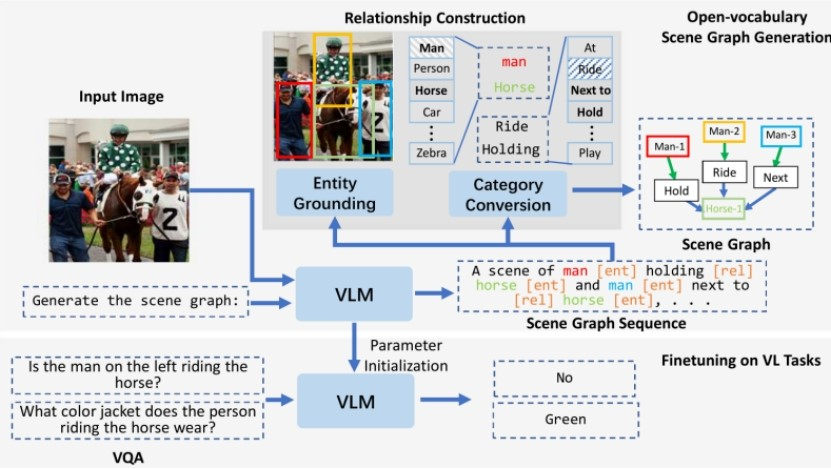
\includegraphics[width=0.7\textwidth]{img/pgsg.jpg}
  \caption{overall pipeline of our PGSG}
\end{figure*}


The PGSG framework comprises three main components:

\textbf{Scene graph prompting}: This component generates sequence representations with relationship-aware tokens, effectively guiding the VLM in capturing relevant visual relationships.

\textbf{Pretrained VLM generating scene graph sequences}: The pretrained VLM generates corresponding scene graph sequences for each input image, translating visual information into structured graph formats.

\textbf{Relationship construction module}: This plug-and-play module uses relationship triplets for entity localization and category conversion. Entity localization predicts entity bounding boxes using an encoder-decoder architecture, while category conversion predicts the transformation from vocabulary space to category space, ultimately generating the output scene graph.


\begin{figure}[h]
    \centering
    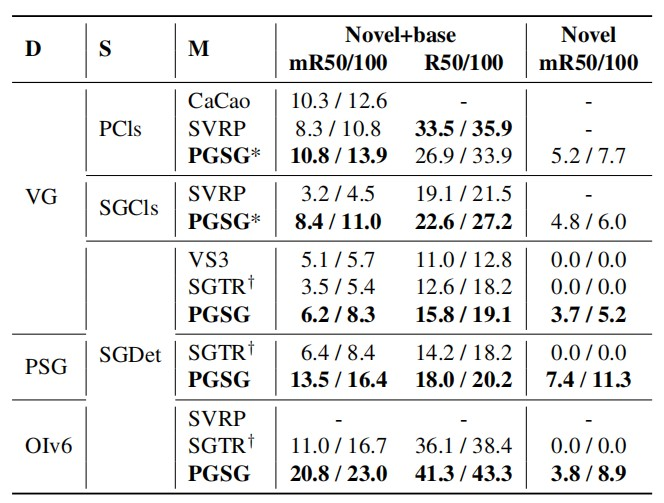
\includegraphics[width=0.5\textwidth]{img/result1_1.jpg} % Adjust the width as needed
    \caption{The open-vocabulary scene graph generation on VG, PSG, and OIV6 datasets}
    \label{fig:pgsg}
\end{figure}


The authors validate their framework on three SGG benchmark datasets \ref{fig:pgsg} (Panoptic Scene Graph, OpenImages-V6, and Visual Genome), achieving state-of-the-art performance. Additionally, they apply the SGG-based VLM to various vision-language tasks such as visual question answering, image captioning, and visual grounding, demonstrating consistent performance improvements. This highlights the effectiveness of their relationship knowledge transfer paradigm in enhancing the interpretability and functionality of vision-language systems.

In summary, this paper proposes a new framework based on generative VLMs to address the general open-vocabulary SGG problem. It introduces scene graph prompting and a plug-and-play relationship-aware transformation module, enabling more efficient model learning and application. The framework demonstrates significant performance improvements in various downstream vision-language tasks, providing new directions and ideas for future research in open-vocabulary visual perception.


\begin{figure*}[h]
  \centering
  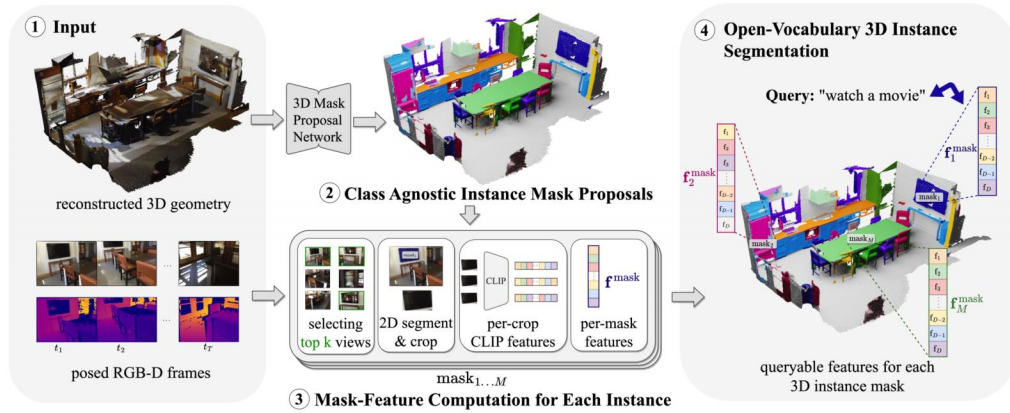
\includegraphics[width=0.7\textwidth]{img/openmark.png}
  \caption{overview of OpenMask3D approach}
\end{figure*}

\subsection{Open-Vocabulary 3D Instance Segmentation}

The paper "OpenMask3D: Open-Vocabulary 3D Instance Segmentation" introduces an innovative technique for open-vocabulary 3D instance segmentation grounded in open-vocabulary visual perception. Traditional 3D instance segmentation methods are constrained to recognizing only predefined object categories that are annotated in the training datasets. This limitation hinders their effectiveness in real-world applications where new and unseen objects frequently appear.

OpenMask3D addresses this limitation through a zero-shot approach, enabling the segmentation of 3D instances based on open-vocabulary descriptions. This method can handle queries that describe previously unseen or novel object attributes, such as geometric shapes, uses, and materials. By doing so, OpenMask3D extends the capabilities of instance segmentation beyond the predefined concepts typically encountered in training data.



OpenMask3D consists of three computational stages:

\textbf{Instance Mask Proposal}: Utilizing a pretrained 3D instance segmentation model’s mask module, OpenMask3D computes category-agnostic instance mask proposals. This step generates initial masks that are not tied to specific object categories, providing a flexible foundation for further processing.

\textbf{Mask Feature Computation}: For each predicted instance mask, OpenMask3D calculates a task-agnostic feature representation using the CLIP model. This process involves selecting the top-k views of the object, obtaining multi-level cropped images, and extracting CLIP features to create a comprehensive feature representation for each mask. This approach ensures that the feature representation captures various aspects of the object from different perspectives.

\textbf{Concept Query Computation}: The final stage involves computing the concept query to obtain the 3D instance segmentation from the previously computed features. This stage leverages the rich, task-agnostic features to match and retrieve object instances based on the similarity to the provided query.


Distinct from existing point-based methods, OpenMask3D emphasizes instance-based feature computation. This focus enhances the system's ability to retrieve object instance masks effectively based on the similarity of features to the query, allowing for more accurate and flexible instance segmentation.

\begin{figure}[h]
    \centering
    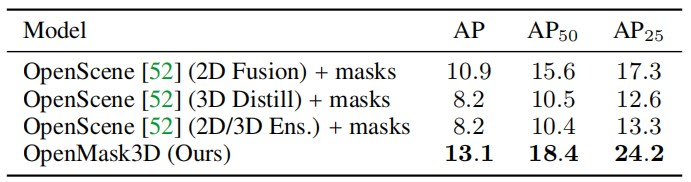
\includegraphics[width=0.5\textwidth]{img/result2_1.jpg}
    \caption{3D instance segmentation results on the Replica dataset}
    \label{fig:Replica}
\end{figure}

\begin{figure*}[h]
    \centering
    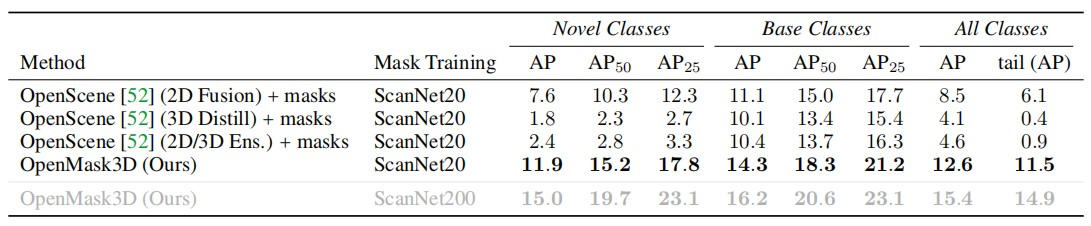
\includegraphics[width=0.9\textwidth]{img/result2_2.jpg}
    \caption{3D instance segmentation results on the ScanNet200 dataset}
    \label{fig:ScanNet}
\end{figure*}

\begin{figure*}[h]
  \centering
  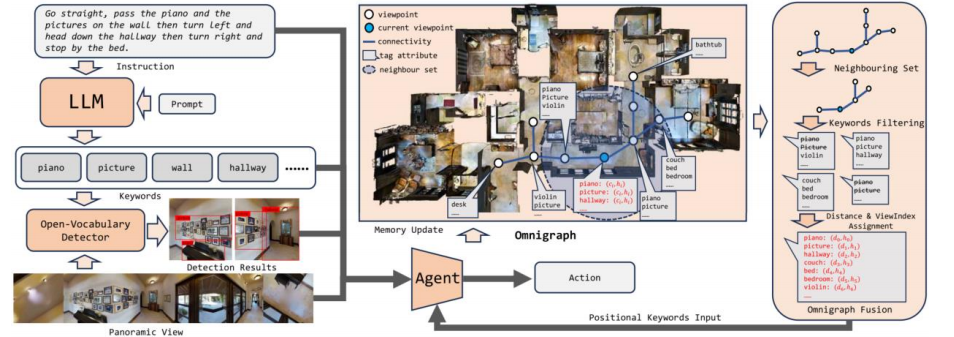
\includegraphics[width=0.8\textwidth]{img/over.png}
  \caption{overview of OVER-NAV method}
\end{figure*}


The authors validate the effectiveness of OpenMask3D on the Replica \ref{fig:Replica} and ScanNet200 \ref{fig:ScanNet} datasets. The results demonstrate that OpenMask3D outperforms existing methods, particularly in handling long-tail distributions of object categories. Qualitative experiments further showcase its capability to segment objects based on diverse attributes and free-form queries, underscoring its versatility and robustness in real-world scenarios.

In summary, similar to the PGSG approach, OpenMask3D leverages vision-language models to transcend the limitations of closed-vocabulary systems. This technique exemplifies the synergistic role of vision-language model methods in advancing open-vocabulary visual perception. Notably, OpenMask3D is the first zero-shot 3D instance segmentation method, significantly broadening the spectrum of recognizable object categories. This advancement enhances the ability of robots to interact with and navigate through unknown environments. It aligns with the objectives of "OVER-NAV," which also improves vision-language navigation through open-vocabulary detection. Together, these methods demonstrate substantial applicability in dynamic and unstructured environments, paving the way for more intelligent and adaptable robotic systems.


\subsection{Vision-and-Language Navigation}

The paper "OVER-NAV: Elevating Iterative Vision-and-Language Navigation with Open-Vocabulary Detection and Structured Representation" introduces a groundbreaking framework for vision-and-language navigation (VLN), termed OVER-NAV. VLN focuses on developing intelligent agents capable of navigating unfamiliar environments by following natural language instructions.

Traditional VLN benchmarks often overlook the agent's memory capabilities, thereby failing to fully leverage cumulative navigation information. While iterative vision-and-language navigation (IVLN) introduces the concept of long-term memory, it still grapples with the challenges of utilizing highly unstructured navigation memory and sparse supervision signals. The OVER-NAV framework effectively addresses these challenges by integrating large language models (LLMs) and open-vocabulary detection (OVD). This integration allows for the extraction and fusion of multimodal information, leading to the construction of a structured memory known as Omnigraph. This significantly enhances the navigation agent’s capability to operate in unseen environments.





The core of the OVER-NAV framework is constructing Omnigraph through OVD. The process includes:

\textbf{Keyword extraction}: LLMs are employed to extract keywords from each navigation instruction. This step ensures that the essential components of the instructions are identified and isolated for further processing.


\textbf{Keyword detection}: As the agent traverses the environment, it continually sends the extracted keywords along with observations made along its path to the OVD. The OVD then detects relevant elements within the environment corresponding to the keywords.

\textbf{Omnigraph construction}: The results from the keyword detection process are stored within the Omnigraph. This structured memory aids the agent in recalling and utilizing parts of the environment’s observations, thus facilitating more informed decision-making.


\textbf{Navigation decision-making}: The real-time computation of scene memory graph information involves feeding the Omnigraph-generated keywords as a text modality into the VLN agent program. This allows the agent to predict navigation actions with greater accuracy in both continuous and discrete environments.


\begin{figure*}[h]
    \centering
    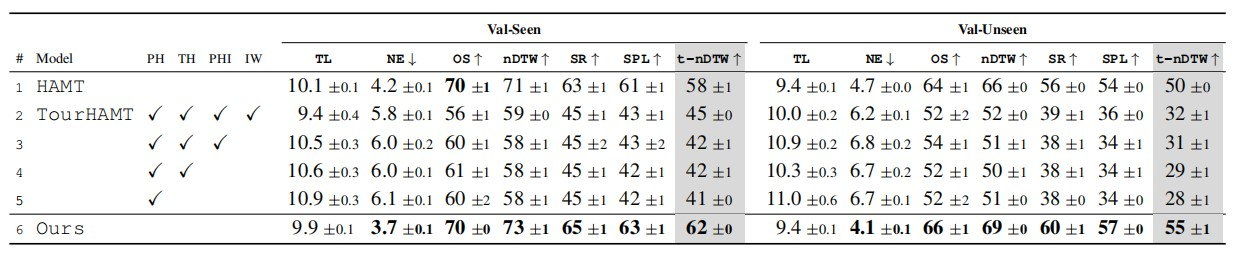
\includegraphics[width=0.8\textwidth]{img/result3_1.jpg} % Adjust the width as needed
    \caption{comparison between OVER-NAV, HAMT and TourHAMT on IR2R}
    \label{fig:IR2R}
\end{figure*}
\begin{figure*}[h]
    \centering
    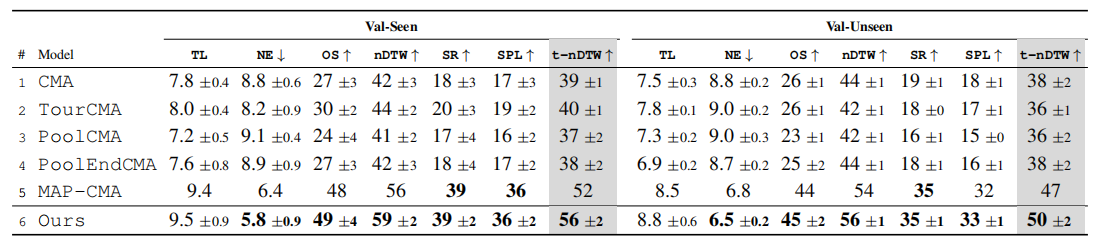
\includegraphics[width=0.8\textwidth]{img/result3_2.jpg} % Adjust the width as needed
    \caption{The performance of OVER-NAV on IR2R-CE}
    \label{fig:IR2R-CE}
\end{figure*}

Experimental results demonstrate the superior performance of OVER-NAV on challenging benchmarks such as IR2R \ref{fig:IR2R} and IR2R-CE \ref{fig:IR2R-CE}. The framework also proves effective in discrete environments, as evidenced by its performance on the REVERIE benchmark. Moreover, the method’s effectiveness is validated when applied to HAMT and MAP-CMA base models, showcasing its versatility and robustness.

In summary, OVER-NAV introduces an innovative framework that incorporates LLMs and OVD into the IVLN paradigm. By introducing a structured representation encoded within Omnigraph, OVER-NAV effectively integrates multimodal information. This leads to significant performance improvements in both discrete and continuous environments, underscoring its potential for advancing the field of vision-and-language navigation.